% [6~v\textsuperscript{o}]
\pstart%
Jam \setline{9}foramina duo ad nares et unum ad palatum ex cerebro maxime conspicua et aperta erant, et palatum ab isto foramine ad dentes erat quibusdam rimis quasi serratum, quae factae videbantur flatu ex cerebro in palatum alliso:
Os autem maxime apertum aquam cui innatabat non poterat non admittere, habebatque item duo foramina in gutture, gulam scilicet
\edtext{et arteriam asperam,}{\lemma{scilicet}\Bfootnote{\textit{(1)}\ et aspe \textit{(2)}\ et arteriam asperam, \textit{L}}}
quae semper aperta videbantur nec epiglottidem notavi, sed immisso per os stylo recta in gulam ivit, cum nihilominus adhuc pateret arteria; jam liquore glutinoso et multo crassiore quam ille cui innatabat foetus stomachus implebatur; unde jejuna intestina alba erant; alia non magis crassa sed nigriora erant; podex denique ni fallor semper patens, sphinctere nondum facto, et intestinum rectum album erat, ut appareret nihildum per istud, quam flatum et aquam limpidam exiisse.
\pend%
\pstart%
%\begin{wrapfigure}[7]{l}{0.28\textwidth}
%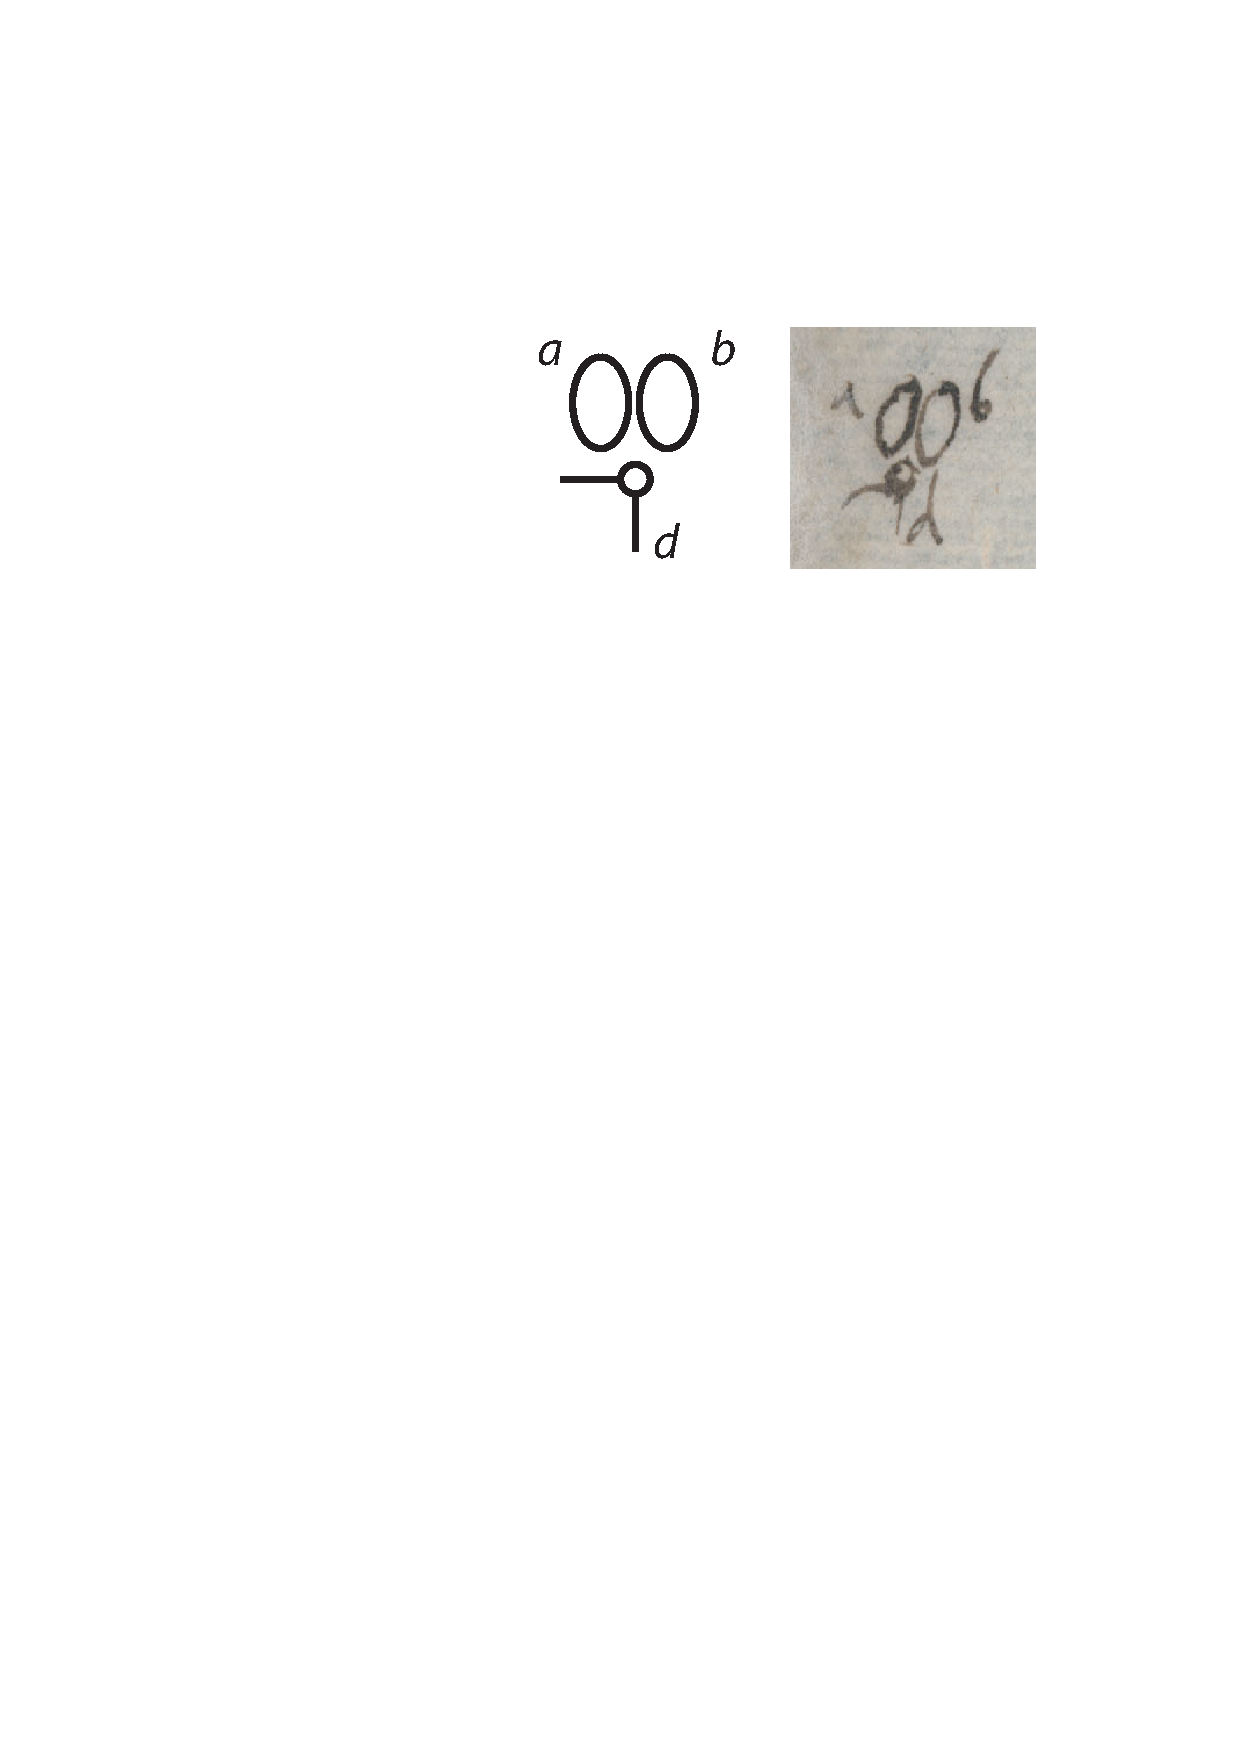
\includegraphics[trim = 0mm -3mm -5mm 0mm, clip, width=0.28\textwidth]{images/lh0040104b_006v1.pdf}\\
%\centering [\textit{Fig. 10}]
%%\caption{Bildbeschreibung}
%\end{wrapfigure}
Cerebrum amplum erat et in tres partes $a.$ $b.$ $c$ ita divisum, ut
\edtext{[earum]}{\lemma{eorum}\Bfootnote{\textit{L \"{a}ndert Hrsg.}}}
unionem videre nequiverim, medulla spinae $d$ exigua:
cor nucis avellanae cum putamine magnitudinem aequabat nec cum pericardio majus erat uno ex ventriculis cerebri; pericardium durum erat imo durissimum; nullum dissepimentum notavi sed diaphragma erat plane
formatum, pulmones erant maxime rubri, nec solidi, sed instar sanguinis concrescentis, item hepar sed magis nigricans; a dextro cordis sinu cavae truncus descendens a sinistro ascendens oriebatur. Renes erant maximi et nigricantes, aorta descendens etiam maxima, rami ex illa ad renes maximi; ureteres a renibus ad imam partem urachi insignes. Vesica autem nulla sed urachus latissimus, instar cuculli vel infundibuli,
\edtext{arteriae umbilicales maximae;}{%
\lemma{arteriae}\Bfootnote{%
\textit{(1)}\ ascendentes maximae %
\textit{(2)}\ umbilicales maximae; \textit{L}}} et aortae descendentis ramis quibusdam inserebantur grandiores quanquam et hi essent insignes stylumque admitterent.
Renes non erant aequaliter siti, sed uter altior, non notavi testes albi satis conspicui, etiam intra corpus natabant. Lien maxime vegetum, et ex
\edtext{rubro splendidissimo}{\lemma{rubro}\Bfootnote{\textit{(1)}\ albo \textit{(2)}\ splendidissimo \textit{L}}}
quasi caeruleum stomacho adhaerebat.
\pend%
\vspace{1em}
\pstart
\centering
\noindent
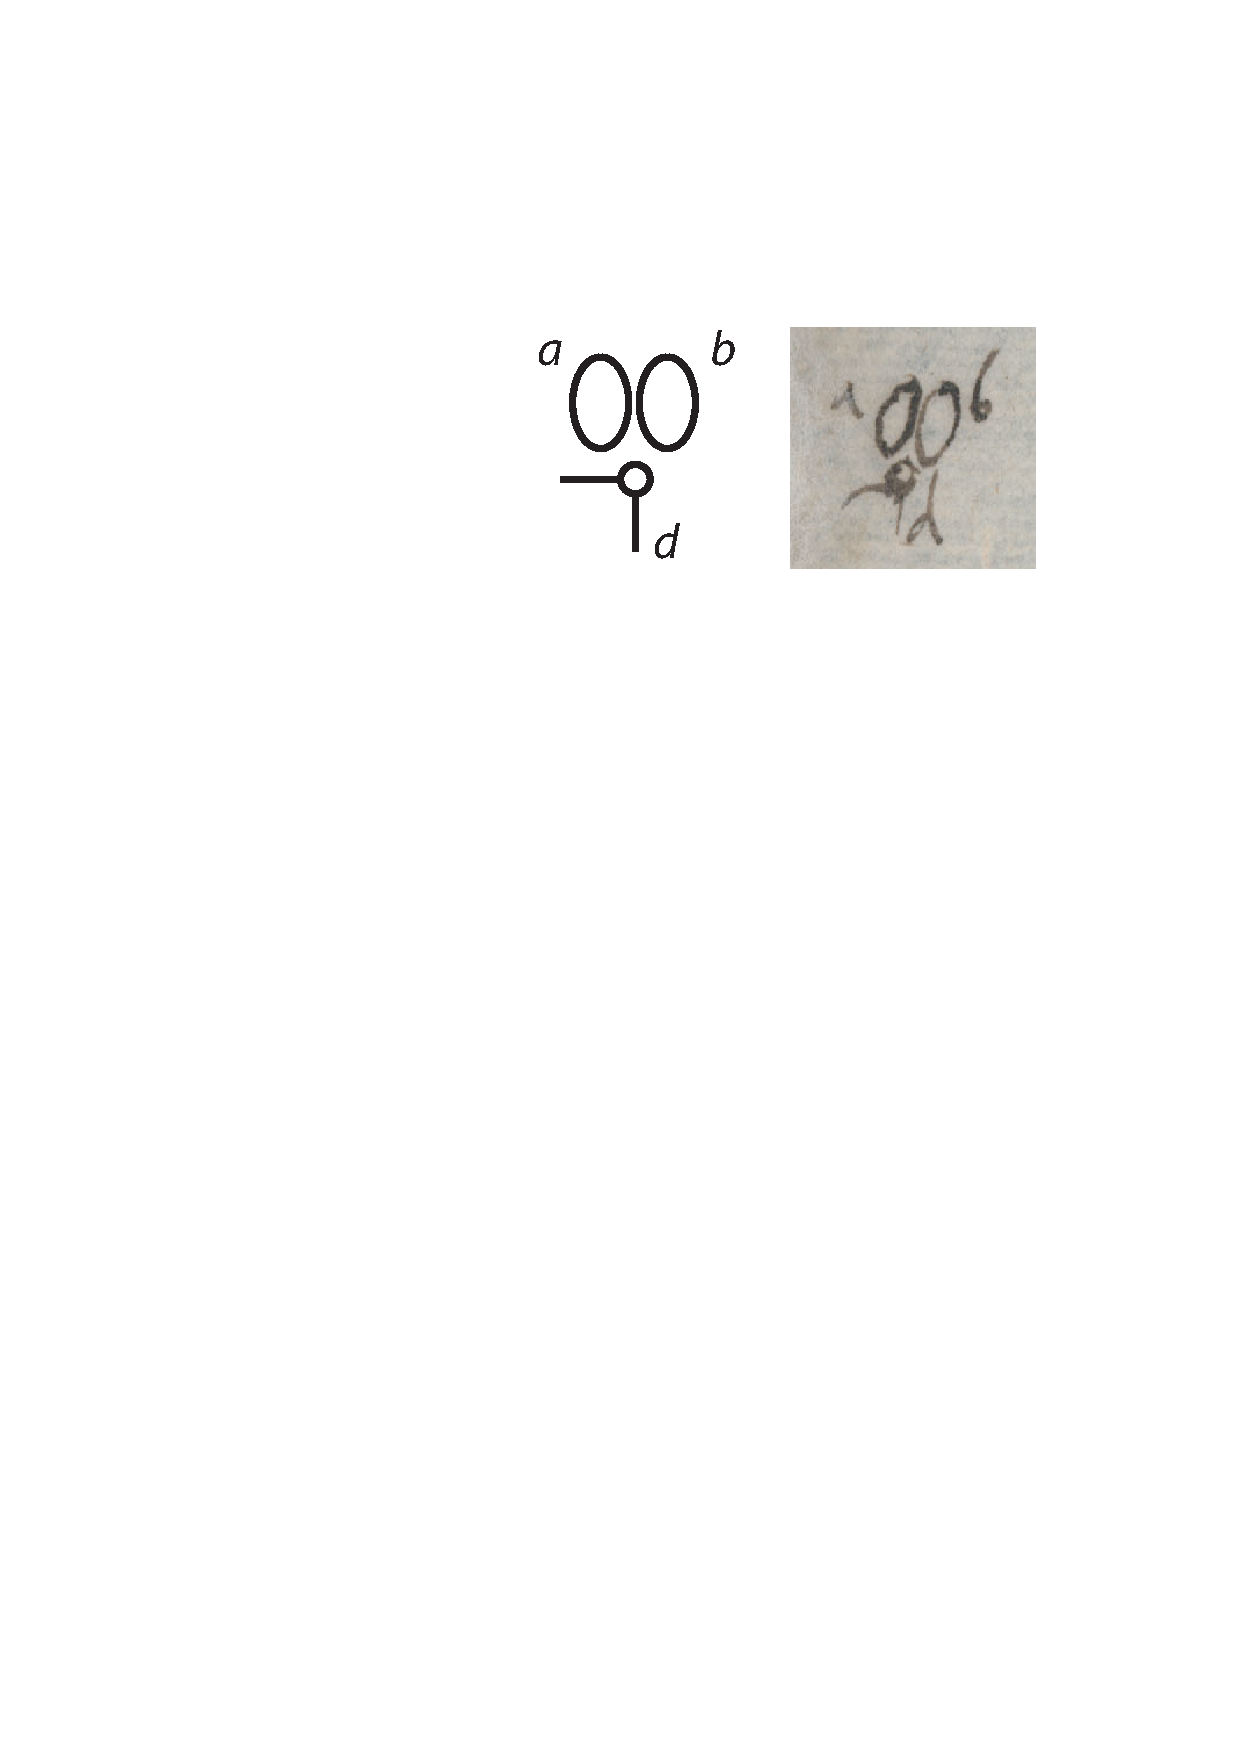
\includegraphics[trim = 0mm -3mm -5mm 0mm, clip, width=0.28\textwidth]{images/lh0040104b_006v1.pdf}\\
\centering [\textit{Fig. 10}]
%%\caption{Bildbeschreibung}
\pend
\vspace{1em}
\pstart%
In \setline{11}\edtext{%
vitulo ad me allato eadem die qua natus est; cumque certus essem, eum nihil unquam edisse; mirum dictu foenum in ore, in gutture, et ventriculo habebat, etiam tantae longitudinis, quantae est manus: in aliis vero intestinis stercus erat viride in podice et recto intestino erat flavescens, adeo ut non modo certum esset, illum antequam nasceretur comedisse, sed etiam ex matris oeso$\phi$ago sive ventriculo per venas ad uterum usque paleas et indigestum alimentum defluxisse, ibique a vitulo exceptum fractis scilicet omnibus membranis ipsum involventibus, neque enim per umbilicum paleae transire potuissent ad gulam, cum praesertim in vena
\edtext{[umbilicali]}{\lemma{umbilicari}\Bfootnote{\textit{L \"{a}ndert Hrsg.}}}
nihil appareret: in arteriis autem umbilicalibus erat sanguis concretus; ren sinister nulli loco fixus haerebat, sed quasi natabat in corpore.
Uterus (erat enim foemina) habebat cornua utrinque reflexa ni fallor supra arterias umbilicales utrinque, hancque puto rationem esse cur cornua
\edtext{[flexa]}{\lemma{facta}\Bfootnote{\textit{L \"{a}ndert Hrsg.}}}
sint, eique proxime testes adhaerebant; stabatque intra vesicam et rectum intestinum hepar fere totum erat in latere dextro magis etiam quam in paulo grandioribus, lien vero non erat adeo incurvum; incipiebat tamen.%
}{\lemma{}\Afootnote{\textit{Absatz am Rand markiert und mit folgendem Vermerk versehen}: Haec omnia in Manuscripto erant deleta rursus.\vspace{-8mm}}}%
\pend%
%
\pstart%
Uteri cornua sursum versus umbilicum reflectuntur et in praegnantibus foetus est in ventris capacitate infra cornua, unde facile est noscere quodnam sit dextrum cornu, quod sinistrum, etiam in vulva excisa:
Uterus $af$ non erat plane
\edtext{perforatus, nisi}{\lemma{perforatus,}\Bfootnote{\textit{(1)}\ sed \textit{(2)}\ nisi \textit{L}}}
usque ad $b,$ inde in duos ramos dividebatur, ita ut $bf$ esset paries utrique ramo communis $fc$ cornu, et $d$ testis.
Intus tota vulva erat exiguis glandulis albis exigui pisi magnitudine disseminata usque ad extremitatem cornuum.
\pend%
\pstart%
In vesica vix patebant ureterum meatus, patebant tamen, et stylum vitreum admittebant.%
\edtext{}{\lemma{}\Afootnote{\textit{Am unteren Rand von Bl. 6~v\textsuperscript{o}:} Nihil deest.}}
[7~r\textsuperscript{o}]
%\pend%
%\newpage% PR: Rein provisorisch !!!
%\vspace*{1.0em}% PR: Rein provisorisch !!!
%\count\Bfootins=1500
%\count\Cfootins=1500
%\count\Afootins=1500